
\begin{tikzpicture}
    \node [examplebox] (box){
        \begin{minipage}{0.5\textwidth}
            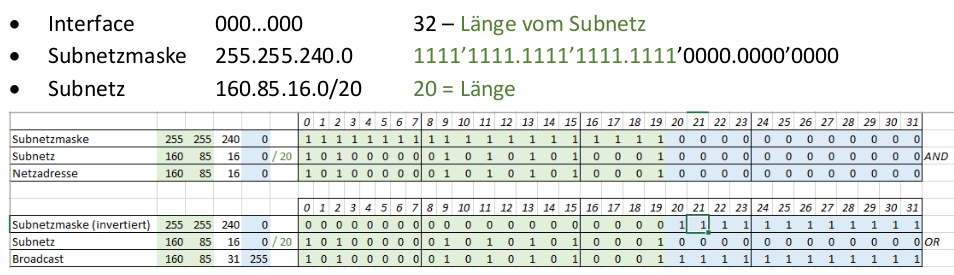
\includegraphics[scale=0.425]{img/ipaddressierung.png}
        \end{minipage}
    };
    \node[exampletitle, right=8pt] at (box.north west) {Addressierung IPv4 Beispiel:};
\end{tikzpicture}



\begin{tikzpicture}
    \node [examplebox] (box){
        \begin{minipage}{0.5\textwidth}
            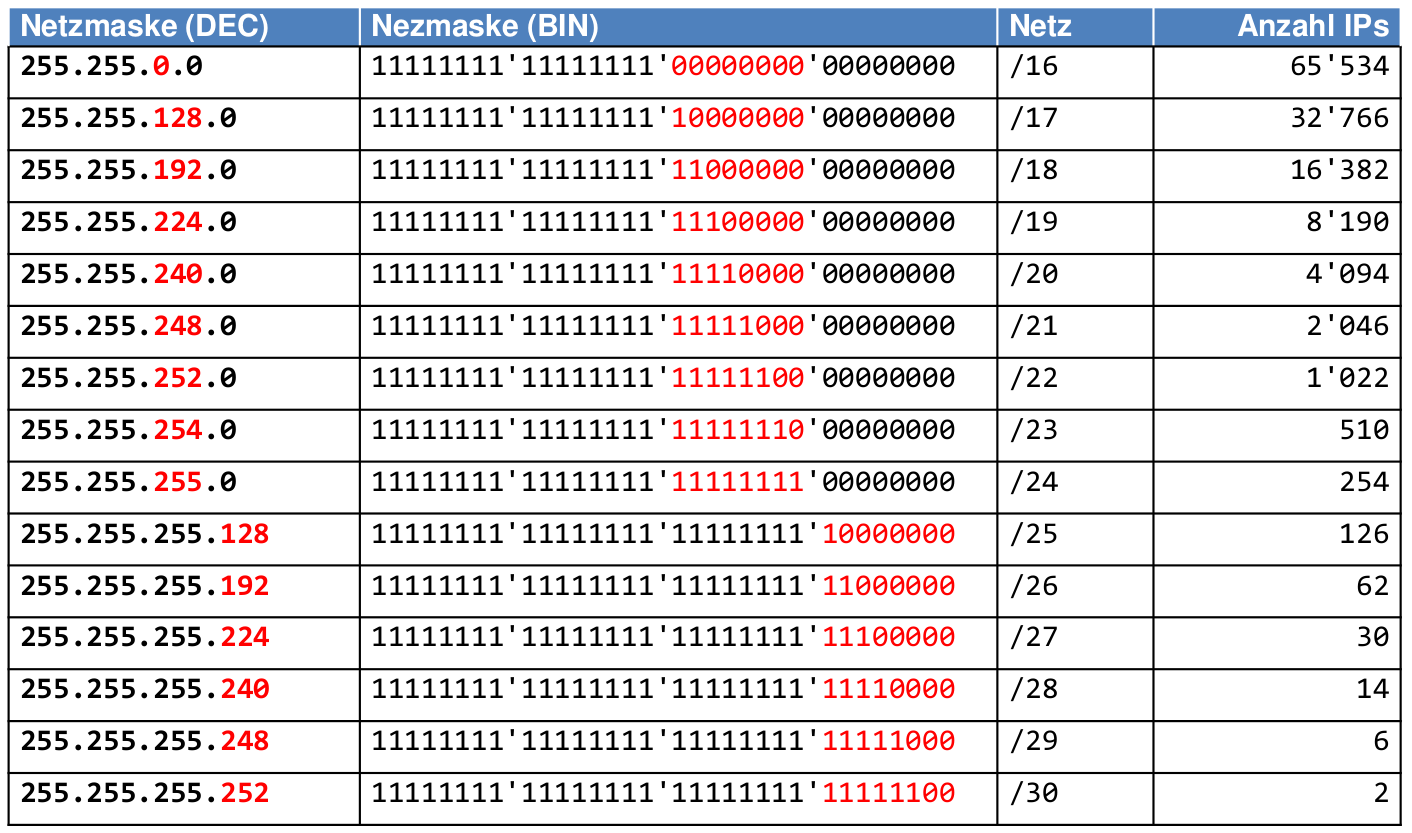
\includegraphics[scale=0.285]{img/subnetzmasken.png}
        \end{minipage}
    };
    \node[exampletitle, right=8pt] at (box.north west) {IP Subnetzmasken};
\end{tikzpicture}




\begin{tikzpicture}
    \node [examplebox] (box){
        \begin{minipage}{0.5\textwidth}

        \end{minipage}
    };
    \node[exampletitle, right=8pt] at (box.north west) {Subnetze Berechnen};
\end{tikzpicture}


\begin{tikzpicture}
    \node [examplebox] (box){
        \begin{minipage}{0.5\textwidth}

        \end{minipage}
    };
    \node[exampletitle, right=8pt] at (box.north west) {Routing Table};
\end{tikzpicture}


\begin{tikzpicture}
    \node [examplebox] (box){
        \begin{minipage}{0.5\textwidth}

        \end{minipage}
    };
    \node[exampletitle, right=8pt] at (box.north west) {ARP Table};
\end{tikzpicture}


